\chapter[Limite, continuité et différentiabilité]{Limite, continuité et différentiabilité des fonctions de plusieurs variables}



%%%%%%%%%%%%%%%%%%%%%%%%%%%%%%%%%%%%%%%%%%%%%%%%%%%%
\section{Limites de fonctions}
%%%%%%%%%%%%%%%%%%%%%%%%%%%%%%%%%%%%%%%%%%%%%%%%%%%%

%En particulier 

Soit $E$ et $F$ deux $\R$ espaces vectoriels de dimension finie munis des normes $\norm{\cdot}$ et $\norm{\cdot}'$ respectivement.

\sld{\vfill\pagebreak[5]}%%%%%%%%%%%%%%%
\subsection{Définition}

\begin{definition}[(Limite de fonction)]
    Soit $f:\D\to F$ une fonction définie sur $\D \subset E$ et $a\in E$ un point adhérent à $\D$ (\ie $a\in \bar{\D}$). On dit que $f$ admet une limite $\ell \in F$ en $a$ si pour tout $\varepsilon>0$ il existe $\alpha>0$ tel que $\forall x \in D$, $\norm{x - a} < \alpha \Rightarrow  \norm{f(x) - \ell}' < \varepsilon$.  
\end{definition}

\begin{center}
    \begin{tabular}{c}
                %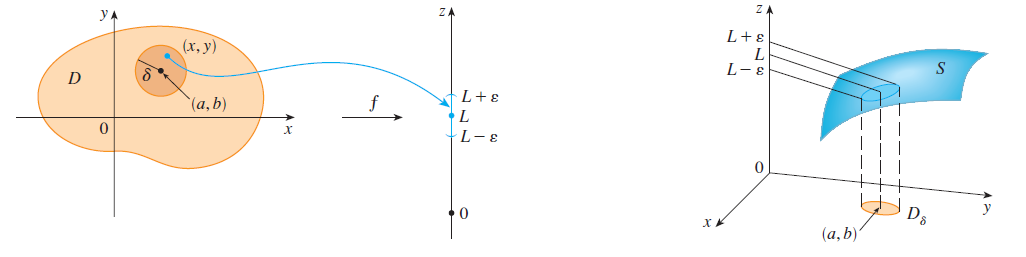
\includegraphics[height=4cm]{./figures/limites_fun.png} \\

        \begin{tikzpicture}[ inner sep=0pt, outer sep=0pt]
            \def\Ox{-.5}
            \def\Imm{6.7}

            \coordinate (a) at (1,.4);
            \coordinate (fa) at (\Imm,1.3);
%axis
            \draw[thick, ->] (5,\Ox) -- node[above=3pt]{$f$} (6,\Ox);
            \draw[thick, ->] (\Imm,-2) -- (\Imm,2.3) node[above=1pt]{$z$};
            \draw[thick,->] (-3,\Ox) -- (4.3,\Ox) node[right=1pt, align=center] {$x$};
            \draw[thick,->] (0,-2) -- (0,2.3) node[above=1pt, align=center]{$y$} ;

            \begin{scope}[shift={(-2.5,2.5)},yscale=-1, scale=.02,]% layer1
                \path[draw=black,fill=green!50,fill opacity=.5,line width=0.915pt] (178.5312,69.9127) .. controls
                (154.7870,70.8770) and (131.0277,74.6352) .. (108.0470,82.6561) .. controls
                (96.9982,86.5932) and (86.1758,91.8084) .. (76.0259,98.7746) .. controls
                (67.8519,104.3691) and (59.9368,111.3314) .. (54.3650,121.1149) .. controls
                (52.1121,125.0658) and (50.3159,129.5092) .. (49.5584,134.3701) .. controls
                (48.3882,141.3583) and (49.2405,148.8923) .. (52.0625,155.0442) .. controls
                (56.0017,164.5781) and (62.7703,171.3756) .. (69.6370,177.0843) .. controls
                (80.9677,186.5254) and (93.6757,192.7324) .. (106.5445,197.5259) .. controls
                (115.7650,200.8851) and (125.1063,203.9008) .. (134.6613,205.0386) .. controls
                (138.6547,205.5173) and (142.8306,205.6972) .. (146.6654,203.9441) .. controls
                (150.1620,202.2792) and (152.6802,198.1257) .. (153.6855,193.5226) .. controls
                (155.3725,186.1698) and (155.4494,178.4112) .. (156.3713,170.8696) .. controls
                (157.2246,163.3019) and (158.7144,155.4868) .. (162.4375,149.4042) .. controls
                (166.0203,143.5149) and (171.8849,140.6317) .. (177.5437,140.8216) .. controls
                (185.6612,141.0665) and (193.1513,145.7111) .. (200.3563,150.1545) .. controls
                (213.5857,159.0623) and (225.7975,170.3354) .. (239.1311,178.9973) .. controls
                (248.1509,184.8771) and (257.7401,189.7005) .. (267.7958,191.3247) .. controls
                (275.9187,192.5503) and (284.3847,191.2698) .. (291.7804,186.5352) .. controls
                (300.6037,181.2603) and (308.8903,174.3200) .. (316.0312,165.7112) .. controls
                (320.8129,159.3821) and (324.6085,151.2633) .. (325.1413,142.2235) .. controls
                (325.6608,132.1003) and (321.9023,122.2182) .. (316.2675,115.4782) .. controls
                (307.7707,104.4017) and (296.9194,97.0755) .. (285.8898,91.2797) .. controls
                (265.5053,80.7777) and (243.8324,75.1531) .. (222.0854,72.3046) .. controls
                (207.6225,70.3479) and (193.0654,69.7423) .. (178.5312,69.9127) -- cycle;
            \end{scope}



            \draw[fill=blue!50] (a) circle (.5cm);
            \filldraw[] (a) circle (.5pt) node[left=2pt]{$a$};

%\node[pin=-30:{\small $B(a,r)$}] at ($(a) + (.5,0)$) {};
            \node[pin=-30:{\small $B_a(\alpha)$}] at ($(a) + (-30:.5)$) {};

            \node[] at (-.6,.2) {$\D_f$};

%image
            \draw[blue,thick] ($(a) +(.1,.1)$) edge[out=45, in= 150,->,%looseness=.5
            ] ($(fa) + (0,.2)$);
            \filldraw[] (\Imm,\Ox) node[right=7pt]{0}  circle (1pt);
            \filldraw[blue] (fa) node[right=7pt]{$\ell$}  circle (1pt);
        \node[blue, rotate=90] (peps) at (\Imm,1.3 +.5) {)};
        \node[blue,right=8pt] at (peps) {$\ell+\varepsilon$};
        \node[blue, rotate=90] (meps) at (\Imm,1.3-.5) {(};
            \node[blue,right=8pt] at (meps) {$\ell-\varepsilon$};
        \end{tikzpicture}
        \\
        Illustration de la limite $\ell\in\R$ d'une fonction $f:\R^2\to\R$ en $a$. 
    \end{tabular}
\end{center}

\sld{\vfill\pagebreak[5]}%%%%%%%%%%%%%%%
\begin{remark}
    \begin{enumerate}
        \item La définition précédente ne dépend pas du choix des normes sur $E$ et $F$.
        \item La limite d'une fonction est unique.
    \end{enumerate}
\end{remark}

\begin{definition}[Notation de Landau]	Soient $(E,\snorm{\cdot})$ et $(F,\snorm{\cdot}')$ deux espaces vectoriels normés réels et $f:E\to F$ définie au voisinage de $a\in E$ (c'est à dire au moins sur une boule ouverte $B_r(a)\subset E$) et sauf peut être en $a$. On dit que $f= o(\snorm{x-a}^n)$ au voisinage de $a$ si $\frac{\snorm{f(x)}'}{\snorm{x -a}^n} \to 0$ quand $x\to a$.  
\end{definition}


\sld{\vfill\pagebreak[5]}%%%%%%%%%%%%%%%

\subsection{Calculer des limites en pratique}

\subsubsection{Montrer qu'une fonction n'admet pas de limite en un point}
\begin{proposition}
    [(Caractérisation séquentielle de la limite)]
    Soit $f:\D\to F$ une fonction définie sur $\D \subset E$ et $a\in E$ un point adhérent à $\D$ (\ie $a\in \bar{\D}$).	Les propositions suivantes sont équivalentes:
    \begin{enumerate}
        \item $f$ a pour limite $\ell$ en $a$
        \item pour toute suite $(u_{k})_{k\in\N}$ de $\D$ qui converge vers $a$, la suite $f(u_k)$ tend vers $\ell$.
    \end{enumerate}
\end{proposition}

\begin{proof}
    \pl{\rep{15cm}}
\end{proof}



Pour montrer qu'une fonction n'admet pas de limite, il suffit de trouver deux suites $(u_k)_{k\in\N}$ et $(v_k)_{k\in\N}$ de même limite $a\in\D$ et telles que $(f(u_k))_{k\in\N}$ et $(f(v_k))_{k\in\N}$ possèdent des limites différentes. 

\sld{\vfill\pagebreak[5]}%%%%%%%%%%%%%%%
\begin{exemple}
    \'Etude de la limite en 0 de $f(x,y)= \begin{cases}\frac{xy}{x^2+y^2}, &\text{si $(x,y) \neq (0,0)$} \\ 0, & \text{si $(x,y) =(0,0)$ }\end{cases}$.

    \begin{center}	\begin{tikzpicture}[scale=.5]
            \begin{axis}[,xlabel=$x$,ylabel=$y$]%,xtick=\empty,ytick=\empty,ztick=\empty ]
                \addplot3[surf,samples=50] gnuplot {(x*y) /(x**2 + y**2)};
            \end{axis}
    \end{tikzpicture}\end{center}
    \pl{\rep{3cm}}
\end{exemple}

\sld{\vfill\pagebreak[5]}%%%%%%%%%%%%%%%
\subsubsection{Montrer qu'une fonction admet une limite en un point}

\begin{proposition}
    Soit $f:\D \to F$, $a \in \bar \D $ et $\ell\in F$. S'il existe une fonction %Les propriétés suivantes sont équivalentes:
    $s: \R^+ \to \R^+$ avec $\lim_{t\to 0} s(t) = 0$ telle que pour tout $x\in D$ 
    \[
        \norm{f(x) - \ell}' \leq s(\norm{x-a})
    \]
    alors on a $\lim_{x \to a } f(x) = \ell$.
\end{proposition}

\begin{proof}
    \pl{\rep{5cm}}	
\end{proof}

\begin{remark}
    Pour les fonctions de $\R^2 \to \R$ cette dernière proposition suggère de passer en coordonnées polaires comme dans l'exemple ci dessous.
\end{remark}

\begin{exemple}
    Calcul de limite en pratique: Soit $f: \R^2 \to \R$ la fonction définie par $f(x,y) = \frac{6x^2y}{x^2+y^2}$. Montrons de plusieurs manières que $\lim_{(x,y) \to (0,0)} f(x,y) = 0$.
    \begin{enumerate}
                %\item Soit $\varepsilon>0$. Il faut trouver $r>0$ tel que $\abs{\sqrt{x^2+y^2}}< r $ implique $\abs{\frac{6x^2y}{x^2+y^2}-0} < \varepsilon$. Comme on a $ x^2 +y^2 \geq x^2$ alors $\abs{\frac{6x^2y}{x^2+y^2}} \leq \frac{6x^2\abs{y}}{x^2} = 6 \abs{y} \leq 6\sqrt{x^2+y^2}$. Il suffit alors de prendre $r=\frac{\varepsilon}{6}$. 
        \item \plprof{ Pour tout $(x,y) \neq (0,0)$ on a  $x^2 +y^2 \geq x^2$ et donc 
                \[
                    \abs{\frac{6x^2y}{x^2+y^2}-0} = 6\abs{ y} \leq 6 \sqrt{x^2 + y^2}  \xrightarrow[(x,y)\to (0,0)]{} 0
            \]}\pl{\rep{4cm}}
        \item \plprof{
                Pour démontrer l'existence d'une limite pour une fonction de $\R^2 \to \R$ il est souvent utile de passer en coordonnées polaires pour ramener le calcul d'une limite de fonction de deux variables à celui d'une limite d'une fonction d'une seule variable. Ainsi, pour tout $(x,y) \neq (0,0)$ on a:
                \[
                    \abs{\frac{6x^2y}{x^2+y^2}-0} = \abs{\frac{6 r^2 \cos^2(\theta) r\sin(\theta) }{r^2}} \leq 6 r \xrightarrow[r\to 0]{} 0
            \]}\pl{\rep{4cm}}
    \end{enumerate}

\end{exemple}

\sld{\vfill\pagebreak[5]}%%%%%%%%%%%%%%%
\section{Fonctions continues}

Soient $E$ et $F$ deux $\R$ espaces vectoriels de dimension finie munis des normes $\norm{\cdot}$ et $\norm{\cdot}'$ respectivement. Dans la suite on note $\D$ un domaine de $E$ et $\U$ un ouvert de $E$.

\subsection{Définition et propriétés}

\begin{definition}
    Soit $f:\D\to F$ et $a\in \D$. On dit que $f$ est \emph{continue} en $a$ si 
    \[
    \lim_{\substack{ x\to a \\ x\in \D}} f(x) = f(a).\]
\end{definition}

La continuité est une notion \emph{locale}. On dit que $f$ est continue sur $\D$ si $f$ est continue en tout point de $\D$.

\begin{exemple}
    Si $E = \R^n$ les fonctions polynômiales sont continues. En particulier si $E = \R^2$, $s(x,y) = x+y$ et $p(x,y) = xy$ sont continues sur $\R^2$.	
\end{exemple}

\sld{\vfill\pagebreak[5]}%%%%%%%%%%%%%%%
\begin{defprop}
    Soit $f:\D\to F$ et $a\in \bar \D \setminus \D$. Si $\lim_{x\to a } f(x) =\ell$, la fonction $\tilde f$ définie sur $\D \cup \left\{ a \right\}$ par $\tilde f(a) = \ell$ et $\tilde f(x) = f(x)$ pour tout $x\in\D$ est l'unique fonction continue en $a$ dont la restriction à $\D$ est $f$. On appelle $\tilde f$ le \emph{prolongement par continuité} de $f$ à $\left\{ a \right\}$. 
\end{defprop}

On peut faire le lien entre topologie et continuité:
\begin{theorem}[]
    Soit $f:E \to F $ une fonction continue:
    \begin{enumerate}[label=$(\roman*)$]
        \item si $\mathcal O \subset F$ un ensemble ouvert, alors $f^{-1}(\mathcal O) \subset E$ est un ouvert. 
        \item si $\mathcal F \subset F$ un ensemble fermé,  alors $f^{-1}(\mathcal F) \subset E$ est un fermé. 
        \item si $K \subset E$ un ensemble compact, alors $f(K) \subset F$ est une partie compacte de $F$. \label{weiertrass}
    \end{enumerate}
\end{theorem}

\begin{proof}
    Admis dans ce cours.
\end{proof}

\begin{remark}
    Si $F = \R$, la propriété \ref{weiertrass} implique que $f$ est bornée (et atteint ses bornes) sur $K$. 
\end{remark}

\sld{\vfill\pagebreak[5]}%%%%%%%%%%%%%%%
\subsection{Opérations sur les fonctions continues}

La continuité est stable par les opérations algébriques usuelles:
\begin{proposition} Soient $E,F,G$ trois espaces vectoriels normés et $\D \subset E$: 
    \begin{enumerate}[label=$(\roman*)$]
        \item Addition: $f,g: \D \to F$ continues en $a\in  \D$ alors $f+g$ est continue en $a$ 
        \item Multiplication par un scalaire: $f:\D\to F$ continue en $a$ alors $\lambda f$ est continue en $a$.
        \item Multiplication (cas de $F=\R$): $f,g:\D\to \R$ continues en $a$ alors $fg$ est continue en $a$.
        \item Inverse (cas de $F=\R$): $f:\D\to \R$ continue en $a$ et $f(a) \neq 0$ alors $\frac{1}{f}$ est continue en $a$.
        \item Composition: $f: \D \to F$ et $g: F \to G $. Si $f$ est continue en $a \in \D$ et $g$ est continue en $f(a)\in F$, alors $g\circ f:\D \to G$ est continue en $a$. 
    \end{enumerate}
\end{proposition}

\begin{proof}

\end{proof}

\begin{exemple}
    \plprof{L'application	$f(x,y)= \begin{cases}\frac{xy}{x^2+y^2}, &\text{si $(x,y) \neq (0,0)$} \\ 0, & \text{si $(x,y) =(0,0)$ }\end{cases}$ est continue sur $\R^2\setminus \left\{ (0,0) \right\}$.}
    \pl{\rep{5cm}}
\end{exemple}

\subsection{Fonctions partielles}

Soit  $\mathcal B=(e_1,\cdots,e_n)$ une base de $E$. Pour tout $a \in E$ on note $(a_1,\cdots,a_n)$ les coordonnées de $a$ dans la base  $\mathcal B$.

\begin{definition}
    Soit $f:  E \to F$ et $a = (a_1,\cdots,a_n) \in E$. On définit la $i$-ème application partielle de $f$ en $a$ par
    \begin{align*}
        f^i_a: \R &\to F \\
        t &\mapsto f(a_1,\cdots,a_{i-1}, t, a_{i+1},\cdots,a_n)
    \end{align*}
\end{definition}

\begin{proposition}
    Si $f$ est continue en $a = (a_1,\cdots,a_n) \in E$ chacune de ses applications partielles $f^i_a$ est continue en $a_i\in\R$ avec $i=1,\cdots,n$.
\end{proposition}

%\blanc{5cm}

\begin{remark}
    La réciproque est fausse: la fonction $f(x,y)= \begin{cases}\frac{xy}{x^2+y^2}, &\text{si $(x,y) \neq (0,0)$} \\ 0, & \text{si $(x,y) =(0,0)$ }\end{cases}$
    \pl{\rep{5cm}}	
\end{remark}

\section{Dérivées partielles }


%\blanc{10cm}

Soit $\U$ un ouvert d'un espace vectoriel normé $E$.


\begin{definition}[(Dérivée suivant un vecteur)] 
    Soit $a\in \U$ et $v\in E$ avec $v\neq 0$. On dit que $f$ admet une dérivée en $a$ suivant la direction $v$ si l'application $t\mapsto f(a+tv) $ est dérivable en $t=0$. Dans ce cas on note:
    \[
        D_v f(a) = \lim_{t\to 0} \frac{f(a+tv) - f(a)}{t}.
    \]
\end{definition}
\begin{remark}
    Dans le cas où $F =\R^p$, on a $f = \begin{psmallmatrix}
        f_1 \\ \vdots \\ f_p
    \end{psmallmatrix}$. Et la limite dans la définition précédente est égale à 
    \[
        \lim_{t\to 0} \frac{f(a+tv) - f(a)}{t} =\lim_{t\to 0} 	\frac{1}{t} \begin{pmatrix}
            f_1(a+tv) - f_1(a)\\
            \vdots \\
            f_p(a+tv) - f_p(a)
        \end{pmatrix} \in \R^p
    \]
\end{remark}

\begin{definition}
%[(Dérivées partielles)]
    Soit  $\mathcal B=(e_1,\cdots,e_n)$ une base de $E$. \'Etant donné $a\in \U$, la $i$-ème \emph{dérivée partielle} de $f$ en $a$ est, lorsqu'elle existe, la dérivée de $f$ en $a$ suivant le vecteur $e_i$ avec $i=1,\cdots,n$. On la note $\frac{\partial f}{\partial x_i} (a)$ et on a
    \begin{align*}
        \frac{\partial f}{\partial x_i} (a) & \doteq D_{e_i} f(a) \\ &= \lim_{t\to 0} \frac{f(a+te_i) - f(a)}{t} = \lim_{t\to 0} \frac{f(a_1,\cdots,a_{i}+t,\cdots,a_n) - f(a_1,\cdots,a_i,\cdots,a_n)}{t}.
    \end{align*}
    Si, de plus, $\frac{\partial f}{\partial x_i} (a)$ existe en tout point $a\in \U$, on définit la $i$-ème \emph{fonction dérivée partielle} de $f$ par: 
    \begin{align*}
        \frac{\partial f}{\partial x_i}: \U &\to F \\
        a & \mapsto \frac{\partial f}{\partial x_i} (a).
    \end{align*}
\end{definition}


\begin{exemple}
    Calcul des dérivées partielles de la fonction	\[f(x,y)= \begin{cases}\frac{xy}{x^2+y^2}, &\text{si $(x,y) \neq (0,0)$} \\ 0, & \text{si $(x,y) =(0,0)$ }\end{cases}\]
    \pl{\rep{6cm}}
\end{exemple}

\sld{\vfill\pagebreak[5]}%%%%%%%%%%%%%%%
\section{Fonctions différentiables}

\begin{exemple}
    Retour sur les fonctions réelles dérivables.
    \pl{\rep{8cm}}
\end{exemple}

\subsection{Définition et propriétés}

Soit $E$ et $F$ deux $\R$ espaces vectoriels de dimension finie munis des normes $\norm{\cdot}$ et $\norm{\cdot}'$ respectivement.

\begin{definition}
    [(Différentiabilité en $a$)]
    Soit $f:E \to F$ définie sur un ouvert $\U$ et $a\in\U$. On dit que $f$ est différentiable en $a$ s'il existe une application linéaire $\varphi_a: E \to F$ telle que 
    \[
        \frac{\norm{f(a+h) - f(a) - \varphi_a(h)}' }{\norm{h}} \xrightarrow[\substack{h\to 0_E \\ h\neq 0_E}]{} 0
    \]
    Avec la notation de Landau cela s'écrit:
    \[
        f(a+h) = f(a) + \varphi_a(h) + o(\norm{h}), \quad \text{quand $h\to 0$}
    \]
\end{definition}

\sld{\vfill\pagebreak[5]}%%%%%%%%%%%%%%%
Contrairement aux dérivée partielles ou directionnelles, la notion de différentiabilité implique la continuité:
\begin{proposition}
    Si $f$ est différentiable en $a$ alors $f$ est continue en $a$.
\end{proposition}
\begin{proof}
    \plprof{Comme l'application linéaire $\varphi_a$ est continue car, en dimension finie, la quantité $ \sup_{h\neq 0}\frac{ \norm{\varphi_a(h)}' }{\norm{h}}$ est finie  et $\lim_{\norm{h}\to 0}\varphi_a(h) = 0$.
    }
    \pl{\rep{5cm}}
\end{proof}

\begin{proposition}
    Si $f$ est différentiable en $a$, $f$ admet en $a$ une dérivée suivant tout vecteur $v \neq 0$. De plus, cette dérivée vaut $\varphi_a(v)$.
\end{proposition}

\begin{proof}
    \pl{\rep{5cm}}
\end{proof}

\begin{defprop}
    Si $f$ est différentiable en $a$, l'application linéaire $\varphi_a: E \to F$ est définie de manière unique. Elle est appelée \emph{différentielle} de $f$ en $a$ et est notée $d_a f$.
\end{defprop}

\begin{proof}
    \pl{\rep{4cm}}
\end{proof}

\begin{proposition}
    Soit  $\mathcal B=(e_1,\cdots,e_n)$ une base de $E$ et $h = h_1 e_1 + \cdots + h_n e_n \in E$. Soit $f:E\to F$ une application différentiable en $a\in E$, alors $d_a f(h) = h_1\frac{\partial f}{\partial x_1}(a) + \cdots + h_n \frac{\partial f}{\partial x_n}(a)$	
\end{proposition}

\begin{proof}
    \pl{\rep{4cm}}
\end{proof}

{\bf \sffamily Notation:} Soit $\mathcal B=(e_1,\cdots,e_n)$ une base de $E$. Pour tout $i=1,\cdots,n$, on note  $dx_i: E \to \R $ l'application linéaire duale de $e_i$ définie par 
\[
    dx_i (e_j) = \begin{cases}
        1 & \text{si $i=j$} \\
        0 & \text{sinon}
    \end{cases}
\]
On a alors $dx_i(h)= h_i$ (en d'autres termes $dx_i$ renvoie la $i$-ème coordonnée de $h\in E$ dans la base $\mathcal B = (e_1,\ldots,e_n)$). On note alors
\[
    d_a f = \frac{\partial f}{\partial x_1} (a)dx_1 + \cdots +\frac{\partial f}{\partial x_n}(a) dx_n 
\]

\begin{proposition}[(Cas de $ \boldsymbol {E=\R}$)]
    Soit $f: \R \to F$. La fonction $f$ est différentiable en $a$ si et seulement si $f$ est dérivable en $a$ et alors $d_af$ est définie par:
    \[
        d_af(h) = h f'(a)
    \]
    pour tout $h\in\R$.
\end{proposition}

\begin{proof}
    \pl{\rep{4cm}}
\end{proof}

\begin{remark}
    Si $F=\R^n$ on a alors $f = \begin{psmallmatrix}
        f_1\\ \vdots \\ f_n
    \end{psmallmatrix}$ et  $f'(a) = \begin{psmallmatrix}
        f'_1(a) \\ \vdots \\ f'_n(a)
    \end{psmallmatrix}\in\R^n$
\end{remark}

\begin{proposition}[(Linéarité de la différentielle)]
    Soient $f,g: E \to F$ différentiables en $a\in E$. Pour tout $\lambda,\mu\in\R$ alors $\lambda f + \mu g$ est différentiable en $a$ avec 
    \[
        d_a (\lambda f + \mu g) = \lambda d_a f + \mu d_a g.
    \]
\end{proposition}

\begin{proof}
    \pl{\rep{4cm}}
\end{proof}

\sld{\vfill\pagebreak[5]}%%%%%%%%%%%%%%%
\subsection{Plan tangent}
\begin{proposition}
    Soit $f:\R^2 \to \R$ définie sur un ouvert $\U\subset  \R^n$ et différentiable en $(x_0,y_0) \in \U$. Le plan tangent à $\G_f$ en $(x_0,y_0,f(x_0,y_0))$ a pour équation:
    \[
        L(x,y) = f(x_0,y_0) + (x-x_0) \dpar{f}{x}(x_0,y_0)  + (y-y_0) \dpar{f}{y}(x_0,y_0). 
    \]
\end{proposition}

\begin{remark}
    L'application $L$ est bien définie sur $\R^2$ tout entier.
\end{remark}

\begin{center}
    \begin{tabular}{c}
        {\small \input{../figures/planTangent.tex}}\\
                        %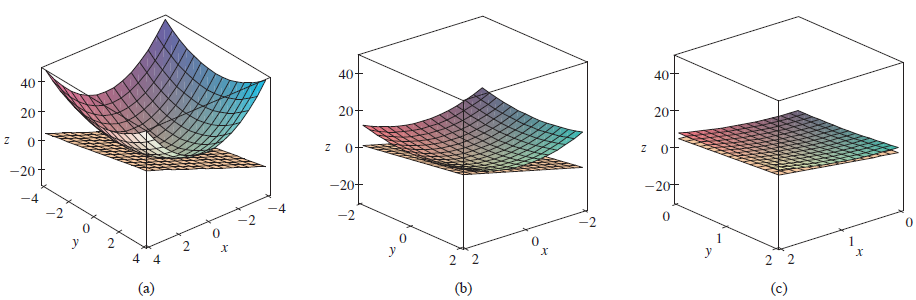
\includegraphics[height=4cm]{./figures/palnTangent.png}\\
                        %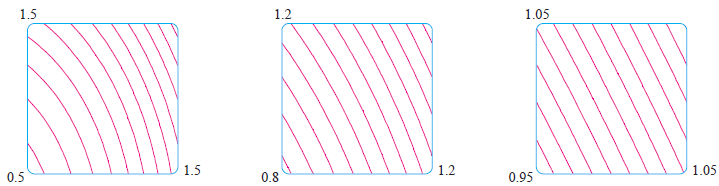
\includegraphics[height=4cm]{./figures/palnTangent_2.png}\\
        \begin{minipage}{.8\textwidth}
            Graphe de la fonction $f(x,y) = x^2 + y^2$ et le plan tangent au point $(-1,-1,f(-1,-1))$. On représente trois niveau de ``zoom'' vers
            ce point. %Si on regarde les courbes de niveau, lorsque on zoom vers ce point les courbes tendent vers des droites parallèles toutes à la même distance les unes des autres.
        \end{minipage}
    \end{tabular}
\end{center}

\sld{\vfill\pagebreak[5]}%%%%%%%%%%%%%%%
\subsection{Vecteur gradient}

Dans cette section, on considère des applications définies sur $\R^n$  et à valeurs réelles. On note aussi $\U$ un ouvert de $\R^n$.

\begin{definition}
    Soit $a\in\U$. On appelle \emph{gradient} de $f: \U \to \R$ en $a$ le vecteur 
    \[
        \nabla f (a) = \begin{pmatrix}
            \frac{\partial f}{\partial x_1}(a) \\
            \vdots\\
            \frac{\partial f}{\partial x_n}(a)

        \end{pmatrix} \in\R^n.
    \]
\end{definition}

\begin{proposition}
    Pour tout $a\in\U$ le gradient est l'unique vecteur de $\R^n$ tel que pour tout $h\in\R^n$ on ait 
    \[
        d_a f(h) = \prs{\nabla f(a) , h}.
    \]
\end{proposition}


%\blanc{5cm}
\begin{center}
        %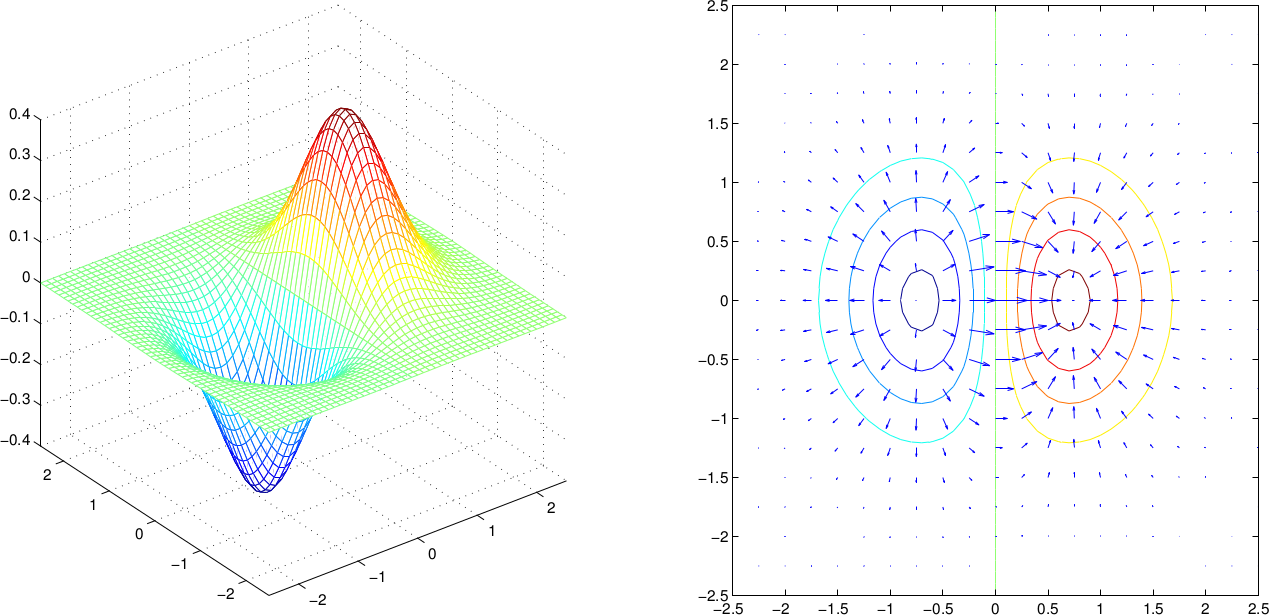
\includegraphics[height=4cm]{./figures/gradient.png}
    \begin{tabular}{c}
        \input{../figures/gradient.tex}
        Graphe, lignes de niveau et gradient de la fonction $(x,y) \mapsto x e^{-x^2 - y^2}$.
    \end{tabular}
\end{center}

\begin{remark}
    \pl{\rep{5cm}}	
\end{remark}


\sld{\vfill\pagebreak[5]}%%%%%%%%%%%%%%%
\subsection{Matrice jacobienne}

\begin{definition}
    Soit $\mathcal B=(e_1,\cdots,e_n)$ une base de $E$. Soit $\mathcal B'=(e'_1,\cdots,e'_p)$ une base de $F$. On suppose $f$ différentiable en $a\in E$. La matrice de l'application linéaire $d_a f:E\to F$ dans les bases $\mathcal B$ et $\mathcal B'$ est appelée \emph{matrice jacobienne} de $f$ en $a$. On la note $\jac_f (a)$.
\end{definition}

\begin{remark}
    On a donc $\jac_f(a) = \operatorname{Mat}_{\mathcal B,\mathcal B'} (d_a f)$
\end{remark}

\begin{proposition}
    On a avec les notations précédentes: 
    \[
        \jac_f(a) =  \begin{pmatrix}
            \frac{\partial f_1}{\partial x_1}(a) & \cdots & \frac{\partial f_1}{\partial x_n}(a) \\
            \vdots & & \vdots \\
            \frac{\partial f_p}{\partial x_1}(a) & \cdots & \frac{\partial f_p}{\partial x_n}(a)\\
        \end{pmatrix} \in \mathcal M_{p,n}(\R)
    \]
    où $n = \dim E$ et $p=\dim F$.
\end{proposition}

\begin{proof}
    \pl{\rep{6cm}}	
\end{proof}

\sld{\vfill\pagebreak[5]}%%%%%%%%%%%%%%%
\begin{definition}
    On suppose que $E=F$ et $\mathcal B = \mathcal B'$. Le déterminant de la matrice $\jac_f(a)$ est alors appelé \emph{jacobien} de $f$ en $a$. 
\end{definition}

{\bf \sffamily Notation:} On note parfaois $\frac{D(f_1,\cdots,f_n)}{D(x_1,\cdots,x_n)} = \det(\jac_f(a))$.
\begin{exemple}
Changement de coordonnées polaires: On a $E=F=\R^2$ et on pose $\psi:]0,+\infty[ \times \R \to \R^2$, $(r,\theta) \mapsto (r\cos\theta,r\sin\theta)$. Calcul du jacobien.
    \pl{\rep{7cm}}
\end{exemple}
